\documentclass[xcolor=svgnames,t,final]{beamer}

\usepackage[T1]{fontenc}
\usepackage[utf8]{inputenc}
\usepackage{lmodern} % Smooth fonts : always use it

\usepackage[french]{babel}

%%%%%%% Page de titre %%%%%%%%%%

\title{Espace Partie 1 \\ Corrigés des exemples du cours}\subtitle{Terminale S 734}
\author[]{Frédéric Junier \thanks{\url{http://frederic-junier.org/} }}
\institute[Lycée du Parc]{Lycée du Parc, Lyon}
\date[]{}

%%%%%%Environnements et symboles mathématiques%%%%

%%%Tableaux de variations %%%%%%%%%%

\usepackage{variations}

%%%%%%%%%%%AmsMaths%%%%%%
\usepackage{mathtools}        %Commandes essentielles, extension d'amsmath
\usepackage{amsfonts,amssymb}  %Principaux symboles
\usepackage{mathrsfs} %Polices calligraphiques
\usepackage{stmaryrd} %Pour les intervalles d'entiers avec \llbracket et \rrbracket
\usepackage[autolanguage, np]{numprint}
%%%%%%%%%%%%Là encore il y a de grosses différences entre le monde anglo-saxon et les francophones.Le séparateur des décimales est un point en anglais et une virgule en français. Leséparateur des milliers est une virgule en anglais et une espace insécable en français. Ilest préférable d’utiliser le package numprint (\usepackage{numprint}) qui associé àfrenchb produira la bonne typographie.
%123456789 = 123456789 \numprint{123456789} = 123 456 789  \numprint{3,1415926535897932384626} = 3,141 592 653 589 793 238 462 6  \numprint{12.34} = 12,34  En plus tu peux préciser les unités de cette façon : \numprint[kg]{12.34} = 12,34 kg ou encore \numprint[\degres C]{22} = 22°C Si tu veux utiliser le raccourci \np{} au lieu de \numprint{}, il te faut charger le package de cette façon : \usepackage[np]{numprint}

\usepackage{bbm, dsfont}   %Fonction indicatrice
\usepackage{esint,esvect}  %Flèches supplémentaires.

%%%%url%%%%

\usepackage{url}

%%%%%%%%%%%Packages spécifiques pour les sorties pdf%%%%%%%%

%%%%Insertion de liens hypertextes %%%%

\usepackage{hyperref}
            
            

%%%%%%%%%%%%Graphiques et Dessins%%%%%%%%%%%%%%

\usepackage{graphicx}		
%\rotatebox[origin=x0x1]{angle}{texte} avec xox1 parmi t (top) l (left) r (right) B (ligne de base) et b (bottomm)
%\resizebox{largeur}{hauteur}{texte} pour faire rentrer u nelement encombrant dans une boite	


%%%%%%%%%%Parametrages Beamer %%%%%%%%%%%%%%%%%

\usetheme{Singapore} % Beamer theme
\usecolortheme[named=Purple]{structure} % Color: latextemplates.com/svgnames-colors
\setbeamercolor{navigation symbols}{fg=black}
\setbeamertemplate{navigation symbols}{\insertframenumber}

%À mettre dans le préambule pour faire apparaitre le plan à chaque section 

\AtBeginSection
{
\begin{frame}
\frametitle{Plan}
\tableofcontents[current, currentsubsection]
\end{frame}
}
 

%%%%%%%%%%%%%%%%%%%%%%%%%%%%
%Le moteur eTeX est aujourd'hui utilisé par toutes les distributions (MikTeX, TeXlive) à la place de l'ancien TeX (en fait, c'est plutôt PDFTeX, le successeur de eTeX, qui est utilisé ; contrairement à ce que son nom indique, il peut produire du dvi). Le fait d'utiliser le moteur eTeX au lieu de TeX donne accès à des choses en plus (par exemple à \middle pour aller avec \left et \right, mais aussi à des commandes bien pratiques comme \numexpr, \dimexpr, \detokenize, etc. ainsi qu'à des ressources supplémentaires, comme plus de compteurs disponibles).

%Lorsqu'on utilise le moteur eTeX, certaines de ces fonctionnalités sont automatiquement accessibles (c'est le cas de \middle, \numexpr, etc.), mais pas d'autres (c'est le cas des compteurs supplémentaires). Pour activer ces fonctionnalités manquantes, on peut charger le package etex.sty. Ainsi, l'utilisation d'etex.sty est une solution courante au problème d'avoir trop de compteurs définis (c'est le cas si on charge ensemble trop de packages du type tikz, pstricks, xymatrix, ...)

%\usepackage{etex}

%%%%%%%%%%%%Graphiques%%%%%%%%%%%%%%
\usepackage{graphicx}	
%\rotatebox[origin=x0x1]{angle}{texte} avec xox1 parmi t (top) l (left) r (right) B (ligne de base) et b (bottomm)	
%\resizebox{largeur}{hauteur}{texte} pour faire rentrer u nelement encombrant dans une boite		
%\usepackage{pstricks,pst-plot,pst-text,pst-tree,pst-eps,pst-fill,pst-node,pst-math,pstricks-add,pst-xkey,pst-blur,pst-coil,pst-grad,pst-eucl}

%\begin{picture}(0,0) permet d'insérer n'importe quoi, n'importe où sans prendre de place (utilie pour annoter une figure en eps)
%Une autre technique est \makebox[0cm][alignement]{texte}
%Exemple:
%\includegraphics[scale=1]{singe.eps}
%\begin{picture}(0,0)
%\put(-27,10){$\sqrt[3]{8}$}
%\end{picture}
\usepackage{pgf,tikz}
\usetikzlibrary{arrows}
\usetikzlibrary{shapes.geometric}
\usetikzlibrary{petri}
\usetikzlibrary{decorations}
\usetikzlibrary{arrows}

%%%%%%%¨Puces%%%%%%%%%%%%
\usepackage{enumerate}


%%%%%%%%%%%%%%%%%%%%%%%%%%%%%%%%%%%%%%%%%%%%%%%%%%%%%%%%%%%%%%%%%%%%%%%%
%%%%%%%%%%%%%%%%%%%%Environnements persos%%%%%%%%%%%%%%%%%%%%%%%%%%%%%%%%
%Syntaxe :
%\newenvironment{nom}[nombre d'args][defaut]{definitions initiales}{definitions finales}
%definitions intiales sont les commandes appelées par \begin{nom}
%Definitions finales sont les commandes appelées par \end{nom}


%%%%%Package listings%%%%%%%%%%%%

\usepackage{listings}
%On utilise l?environnement lstlisting pour insérer
%un code source.
%En plus de l?environnement lstlisting, on peut également utiliser la
%commande \lstinline qui fonctionne comme la commande \verb, en ce
%sens qu?on peut utiliser n?importe quel caractère comme délimiteur. Enfin,
%la commande \lstinputlisting permet de charger un code source depuis
%un fichier externe.
%Il y a deux manières de préciser des options : soit via l?option de l?envi-
%ronnement ou de la commande, soit en utilisant la commande \lstset
%qui permet de définir des options de manière globale.

\lstset{ %
  language=Python,                % the language of the code
  basicstyle=\ttfamily,           % the size of the fonts that are used for the code
  numbers=left,                   % where to put the line-numbers
  numberstyle=\tiny,  % the style that is used for the line-numbers
  %stepnumber=2,                   % the step between two line-numbers. If it's 1, each line 
                                  % will be numbered
  %numbersep=5pt,                  % how far the line-numbers are from the code
  backgroundcolor=\color{white},      % choose the background color. You must add \usepackage{color}
  showspaces=false,               % show spaces adding particular underscores
  showstringspaces=false,         % underline spaces within strings
  showtabs=false,                 % show tabs within strings adding particular underscores
  %frame=single,                   % adds a frame around the code
  rulecolor=\color{black},        % if not set, the frame-color may be changed on line-breaks within not-black text (e.g. comments (green here))
  tabsize=4,                      % sets default tabsize to 2 spaces
  captionpos=b,                   % sets the caption-position to bottom
  breaklines=true,                % sets automatic line breaking
  breakatwhitespace=false,        % sets if automatic breaks should only happen at whitespace
  %title=\lstname,                   % show the filename of files included with \lstinputlisting;
                                  % also try caption instead of title
  breakindent=1cm,
  keywordstyle=\color{blue},          % keyword style
  commentstyle=\color{red},       % comment style
  %stringstyle=\ttfamily\color{green},         % string literal style
  escapeinside={\%*}{*)},            % if you want to add LaTeX within your code
  morekeywords={*,...},              % if you want to add more keywords to the set
  deletekeywords={...}              % if you want to delete keywords from the given language
  upquote=true,columns=flexible,
  frame=lines,
  extendedchars=true,
xleftmargin=1cm,xrightmargin=1cm
}


%\lstset{language=Python,basicstyle=\small , frame=single,tabsize=4,showspaces=false,showtabs=false,showstringspaces=false,numbers=left,numberstyle=\tiny , extendedchars=true}


%%%%%PAckages pour l'environnement algobox%%%%%%%%%%%%%%%%%%%%%%%%%%%%%%%%%%
\usepackage{algorithm}
\usepackage{algpseudocode}



%%%%%%%%%%%%%%%%%%Maths divers%%%%%%%%%%%%%%%%%%%%%%%%%
%Delimiteurs
\newcommand{\delim}[3]{\raise #1\hbox{$\left #2\vbox to #3{}\right.$}}


%%%%%%%%%%%%%Nombres%%%%%%%%%%%%%%%%

%Ensemble prive de...
%\newcommand{\prive}{\boi}%{\backslash}

%Ensembles de nombres%%%%%%%%%%%%%%%%%
\newcommand{\R}{\mathbb{R}}
\newcommand{\N}{\mathbb{N}}
\newcommand{\D}{\mathbb{D}}
\newcommand{\Z}{\mathbb{Z}}
\newcommand{\Q}{\mathbb{Q}}
\newcommand{\C}{\mathbb{C}}
\newcommand{\df}{~\ensuremath{]0;+\infty[}~}
\newcommand{\K}{\mathbb{K}}

%%%%%%%%Arithmetique%%%%%%%%%%
%PGCD, PPCM
\newcommand{\PGCD}{\mathop{\rm PGCD}\nolimits}
\newcommand{\PPCM}{\mathop{\rm PPCM}\nolimits}

%Intervalles
\newcommand{\interoo}[2]{]#1\, ;\, #2[}
\newcommand{\Interoo}[2]{\left]#1\, ;\, #2\right[}
\newcommand{\interof}[2]{]#1\, ;\, #2]}
\newcommand{\Interof}[2]{\left]#1\, ;\, #2\right]}
\newcommand{\interfo}[2]{[#1\, ;\, #2[}
\newcommand{\Interfo}[2]{\left[#1\, ;\, #2\right[}
\newcommand{\interff}[2]{[#1\, ;\, #2]}
\newcommand{\Interff}[2]{\left[#1\, ;\, #2\right]}
%\newcommand\interentiers #1#2{[\! [#1\, ;\, #2]\! ]}
\newcommand{\interentiers}[2]{\llbracket #1\, ;\, #2\rrbracket}
%


%%%%%%%%%%%%%%Nombres complexes%%%%%

\newcommand{\ic}{\text{i}}
%\newcommand{\I}{\text{i}}
\newcommand{\im}[1]{\text{Im}\left(#1\right)}
\newcommand{\re}[1]{\text{Re}\left(#1\right)}
\newcommand{\Arg}[1]{\text{arg}\left(#1\right)}
\newcommand{\Mod}[1]{\left[#1\right]}
%Parties entière, réelle, imaginaire, nombre i
\newcommand{\ent}[1]{\text{E}\left(#1\right)}
\renewcommand{\Re}{\mathop{\rm Re}\nolimits}
\renewcommand{\Im}{\mathop{\rm Im}\nolimits}
\renewcommand{\i}{\textrm{i}}

%%%%%%%%%%%Probabilites et statistiques%%%%%
\newcommand{\loibinom}[2]{\mathcal{B}\left(#1\ ; \ #2 \right)}
\newcommand{\loinorm}[2]{\mathcal{N}\left(#1\ ; \ #2 \right)}
\newcommand{\loiexp}[1]{\mathcal{E}\left(#1\right)}
\newcommand{\proba}[1]{\text{P}\big(#1\big)}
\newcommand{\probacond}[2]{\text{P}_{#2}\big(#1\big)}
\newcommand{\esperance}[1]{\text{E}\left(#1\right)}
\newcommand{\variance}[1]{\text{V}\left(#1\right)}
\newcommand{\ecart}[1]{\sigma\left(#1\right)}
\newcommand{\dnormx}{\frac{1}{\sqrt{2\pi}} \text{e}^{-\frac{x^2}{2}}}
\newcommand{\dnormt}{\frac{1}{\sqrt{2\pi}} \text{e}^{-\frac{t^2}{2}}}
\newcommand{\nbalea}[2]{\reinitrand[first=#1, last=#2, counter=num]  \rand $\thenum$}  %retourne un entier aleatoire antre les bornes #1 et #2 comprises
%Covariance
\newcommand{\cov}{\mathop{\rm cov}\nolimits}
%


%%%%%%%%%%Analyse%%%%%%%%%%%

%%%%%%%%%%%Courbe%%%%%%%%%%%%
\newcommand{\courbe}[1]{\ensuremath{\mathcal{C}_{#1}}}

%%%%%%%Fonction exponentielle%%%%%
\newcommand{\fe}{~fonction exponentielle~}
\newcommand{\e}{\text{e}}

%Fonction cotangente
\newcommand{\cotan}{\mathop{\rm cotan}\nolimits}
%%%%%%%%%%%%%%%%%%%%%%%%%%%%%%%%%%%%%%%%%
%
%Fonctions hyperboliques
\newcommand{\ch}{\mathop{\rm ch}\nolimits}
\newcommand{\sh}{\mathop{\rm sh}\nolimits}


%%%%%%%%%%%%%%Limites%%%%%%
\newcommand{\limite}[2]{\lim\limits
_{x \to #1} #2}
\newcommand{\limitesuite}[1]{\lim\limits
_{n \to +\infty} #1}
\newcommand{\limiteg}[2]{\lim\limits
_{\substack{x \to #1 \\ x < #1 }} #2}
\newcommand{\limited}[2]{\lim\limits
_{\substack{x \to #1 \\ x > #1 }} #2}

%%%%%%%%%%Continuité%%%%%%%%%%%
\newcommand{\TVI}{théorème des valeurs intermédiaires}

%%%%%%%%%%%Suites%%%%%%%%%%%%
\newcommand{\suite}[1]{\ensuremath{\left(#1_{n}\right)}}
\newcommand{\Suite}[2]{\ensuremath{\left(#1\right)_{#2}}}
%

%%%%%%%%%%%%%%%Calcul intégral%%%%%%
\newcommand{\dx}{\ensuremath{\text{d}x}}		% dx
\newcommand{\dt}{\ensuremath{\text{d}t}}		% dt
\newcommand{\dtheta}{\ensuremath{\text{d}\theta}}		% dtheta
\newcommand{\dy}{\ensuremath{\text{d}y}}		% dy
\newcommand{\dq}{\ensuremath{\text{d}q}}		% dq

%%%Intégrale%%%
\newcommand{\integralex}[3]{\int_{#1}^{#2} #3 \ \dx}
\newcommand{\integralet}[3]{\int_{#1}^{#2} #3 \ \dt}
\newcommand{\integraletheta}[3]{\int_{#1}^{#2} #3 \ \dtheta}

%%%%%Equivalent%%
\newcommand{\equivalent}[1]{\build\sim_{#1}^{}}

%o et O%%%%
\renewcommand{\o}[2]{\build o_{#1\to #2}^{}}
\renewcommand{\O}[2]{\build O_{#1\to #2}^{}}



%%%%%%%%%%%%%%%Geometrie%%%%%%%%%%%%%%%%%%%%%%%

%%%%%%%%%%%%%%%Reperes%%%%%%%%%%%%%%
\def\Oij{\ensuremath{\left(\text{O},~\vect{\imath},~\vect{\jmath}\right)}}
\def\Oijk{\ensuremath{\left(\text{O},~\vect{\imath},~ \vect{\jmath},~ \vect{k}\right)}}
\def\Ouv{\ensuremath{\left(\text{O},~\vect{u},~\vect{v}\right)}}
\renewcommand{\ij}{(\vec\imath\, ;\vec\jmath\,)}
\newcommand{\ijk}{(\vec\imath\, ;\vec\jmath\, ;\vec k\,)}
\newcommand{\OIJ}{(O\,;\, I\,;\, J\,)}
\newcommand{\repere}[3]{\big(#1\, ;\,\vect{#2} ;\vect{#3}\big)}
\newcommand{\reperesp}[4]{\big(#1\, ;\,\vect{#2} ;\vect{#3} ;\vect{#4}\big)}

%%%%%%%%%Coordonnees%%%%%%%%%%%%%%
\newcommand{\coord}[2]{(#1\, ;\, #2)}
\newcommand{\bigcoord}[2]{\big(#1\, ;\, #2\big)}
\newcommand{\Coord}[2]{\left(#1\, ;\, #2\right)}
\newcommand{\coordesp}[3]{(#1\, ;\, #2\, ;\, #3)}
\newcommand{\bigcoordesp}[3]{\big(#1\, ;\, #2\, ;\, #3\big)}
\newcommand{\Coordesp}[3]{\left(#1\, ;\, #2\, ;\, #3\right)}

%Symboles entre droites
%\newcommand{\paral}{\sslash}
\newcommand{\paral}{\mathop{/\!\! /}}
%
%%%%%%%%%Produit scalaire, Angles%%%%%%%%%%
\newcommand{\scal}[2]{\vect{#1} \, \cdot \, \vect{#2}}
\newcommand{\Angle}[2]{\left(\vect{#1} \, , \, \vect{#2}\right)}
\newcommand{\Anglegeo}[2]{\left(\widehat{\vect{#1} \, , \, \vect{#2}}\right)}
\renewcommand{\angle}[1]{\widehat{#1}}
\newcommand{\anglevec}[2]{\left(\vec {#1}\, ,\,\vec {#2} \right)}
\newcommand{\anglevecteur}[2]{(#1\, ,\, #2)}
\newcommand{\Anglevec}[2]{(\vecteur{#1}\, ,\,\vecteur{#2})}
\newcommand{\prodscal}[2]{#1 \, \cdot \, #2}

%Arc
%\newcommand{\arc}[1]{\wideparen{#1}}
\newcommand{\arcoriente}[1]{\overset{\curvearrowright}{#1}}
%
%


%%%%%%%%%%%%%%%Normes%%%%%%%%%%%%%%%%
\newcommand{\norme}[1]{\left\| #1\right\|}
\newcommand{\normebis}[1]{\delim{2pt}{\|}{9pt}\! #1\delim{2pt}{\|}{9pt}}
\newcommand{\normetriple}[1]{\left |\kern -.07em\left\| #1\right |\kern -.07em\right\|}
\newcommand{\valabs}[1]{\big| \, #1 \, \big|}
%

%%%%%%%%%%%%%%%%%%%%%%%%%%%Degré%%%%%%
%\newcommand{\Degre}{\ensuremath{^\circ}}
%La commande \degre est déjà définie dans le package babel

%%%%%%%%%%Vecteurs%%%%%%%%%%%
\newcommand{\vect}[1]{\mathchoice%
{\overrightarrow{\displaystyle\mathstrut#1\,\,}}%
{\overrightarrow{\textstyle\mathstrut#1\,\,}}%
{\overrightarrow{\scriptstyle\mathstrut#1\,\,}}%
{\overrightarrow{\scriptscriptstyle\mathstrut#1\,\,}}}



%%%%%%%%%%%%%Algebre%%%%%%%%%%%%%%%


%%%%%%%%%%Systemes%%%%%%%%%%%
%Systemes
\newcommand{\sys}[2]{
\left\lbrace
 \begin{array}{l}
  \negthickspace\negthickspace #1\\
  \negthickspace\negthickspace #2\\
 \end{array}
\right.\negthickspace\negthickspace}
\newcommand{\Sys}[3]{
\left\lbrace
 \begin{array}{l}
  #1\\
  #2\\
  #3\\
 \end{array}
\right.}
\newcommand{\Sysq}[4]{
\left\lbrace
 \begin{array}{l}
  #1\\
  #2\\
  #3\\
  #4\\
 \end{array}
\right.}
%
%

%%%%%%%%%%%%%%%%Matrices%%%%%%%%%%%%%%%%%%
%Comatrice
\newcommand{\com}{\mathop{\rm com}\nolimits}
%
%
%Trace
\newcommand{\tr}{\mathop{\rm tr}\nolimits}
%
%
%Transposee
\newcommand{\transposee}[1]{{\vphantom{#1}}^t\negmedspace #1}
%
%
%Noyau
\newcommand{\Ker}{\mathop{\rm Ker}\nolimits}
%
%

%
%Matrices
\newcommand{\Mn}{\mathcal M_n}
\newcommand{\matrice}[4]{
\left(
 \begin{array}{cc}
  #1 & #2 \\
  #3 & #4
 \end{array}
\right)}

\newcommand{\Matrice}[9]{
\left(
 \begin{array}{ccc}
  #1 & #2 & #3\\
  #4 & #5 & #6\\
  #7 & #8 & #9
 \end{array}
\right)}
\newcommand{\Vect}[3]{
\left(\negmedspace
 \begin{array}{c}
  #1\\
  #2\\
  #3
 \end{array}\negmedspace
\right)}
\newcommand{\Ideux}{\matrice{1}{0}{0}{1}}
\newcommand{\Itrois}{\Matrice{1}{0}{0}{0}{1}{0}{0}{0}{1}}
%
%
%Determinants
\newcommand{\determinant}[4]{
\left|
 \begin{array}{cc}
  #1 & #2 \\
  #3 & #4
 \end{array}
\right|}
\newcommand{\Determinant}[9]{
\left|
 \begin{array}{ccc}
  #1 & #2 & #3\\
  #4 & #5 & #6\\
  #7 & #8 & #9
 \end{array}
\right|}



%%%%%%%%%%%%%%%%%%%%%%%%%%%%%%%%%%%%%%%
%%%%%%%%%%%Commandes Tikz%%%%%%%%%%%%%%%

% Définition des nouvelles options xmin, xmax, ymin, ymax
% Valeurs par défaut : -3, 3, -3, 3
\tikzset{
xmin/.store in=\xmin, xmin/.default=-3, xmin=-3,
xmax/.store in=\xmax, xmax/.default=3, xmax=3,
ymin/.store in=\ymin, ymin/.default=-3, ymin=-3,
ymax/.store in=\ymax, ymax/.default=3, ymax=3,
}
% Commande qui trace la grille entre (xmin,ymin) et (xmax,ymax)
\newcommand {\grille}[1]
{\draw[help lines] (\xmin,\ymin) grid[step=#1] (\xmax,\ymax);}
% Commande \axes
\newcommand {\axes} {
\draw[->,very thick] (\xmin,0) -- (\xmax,0);
\draw[->,very thick] (0,\ymin) -- (0,\ymax);
\draw (\xmax, 0) node[above] {$x$};
\draw (0, \ymax) node[left] {$y$};
}
% Commande qui limite l?affichage à (xmin,ymin) et (xmax,ymax)
\newcommand {\fenetre}
{\clip (\xmin,\ymin) rectangle (\xmax,\ymax);}

%Exemple d'utilisation

%\begin{center}
%\begin{tikzpicture} [xmin=-2,xmax=2,ymin=0,ymax=5]
%\grille{1} \axes \fenetre
%\draw plot[smooth] (\x,\x^2);
%\end{tikzpicture}
%\end{center}


%%%%%%%%%%%%%%%%%%%%%%%%%%%%%%%%%%%%%%%%
%%%%%%%%%%%Fin Commandes Tikz%%%%%%%%%%%%%%%


%%%%%%Cadre Maxima%%%%%%%
\definecolor{labelcolor}{RGB}{100,0,0}


%%%%%%%Symbole pour code calculatrice%%%%%%

%Flèche remplie pour défilement de menu

\newcommand{\flechefillright}{
\begin{tikzpicture}[scale=0.15] \fill (0,0)--(2,1)--(0,2)--cycle;
\end{tikzpicture}}

%%%%%%%%%%%%%Symboles pour calculatrice Casio%%%%
\newcommand{\execasio}{\Pisymbol{psy}{191}} %Retour chariot
\newcommand{\dispcasio}{\begin{pspicture}(.1,.1)\pspolygon*(.1,0)(.1,.1)\end{pspicture}} %Triangle « Disp »
\newcommand{\dispcasiotikz}{\begin{tikzpicture}[scale=0.2]
\fill (0,0) -- (1,0) -- (1,1) -- cycle;
\end{tikzpicture}} %Triangle « Disp »
%
%
%Fleche entre deux lignes, d'apres 'un bon petit' : http://forum.mathematex.net/latex-f6/fleches-entre-deux-lignes-pour-resolution-d-equation-t10283.html#p99817
\newcommand\addnode[1]{\Rnode{#1}{}}
\newcommand\linknode[3]{\ncbar[angleA=0,angleB=0,nodesep=1ex,arm=10ex,offset=-2pt]{->}{#1}{#2}\Aput{\vphantom{x}#3}}

%%%%%Fin des commandes Mathematiques%%%%%%%%

\everymath{\displaystyle}

\begin{document}

\frame{\titlepage}


\begin{frame}
\frametitle{Table des matières}
\begin{itemize}
	\item \hyperlink{exemple1}{Exemple 1}
	\item \hyperlink{exemple2}{Exemple 2}
	\item \hyperlink{exemple3}{Exemple 3}
	\item \hyperlink{exemple4}{Exemple 4}
	\item \hyperlink{exemple5}{Exemple 5}
	\item \hyperlink{exemple6}{Exemple 6}
		\item \hyperlink{exemple7}{Exemple 7}
			\item \hyperlink{exemple8}{Exemple 8}
	
\end{itemize}

\end{frame}
 

 
\begin{frame}
\label{exemple1}
\frametitle{Exemple 1 : Partie 1}

Figure dynamique sur \href{https://www.geogebra.org/m/ahkmk9br}{https://www.geogebra.org/m/ahkmk9br}.


\begin{center}
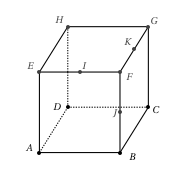
\includegraphics[scale=0.4]{images/exemple1.png}
\end{center}

\begin{itemize}
\pause \item {\color{blue} Question : Les droites $(GF)$ et $(AH)$ sont-elles
   parallèles ? sécantes ? }
\pause \item {\color{red} Réponse : Les droites $(GF)$ et $(AH)$ n'ont pas d'intersection car elles sont dans des plans parallèles $(CGF)$ et $(AEH) $, donc elles ne sont pas sécantes.  Si on avait $(GF)//(AH)$ alors on aurait $(AH)//(EH)$ car $(GF)//(EH)$ puisque $EFGH$ est un carré . On aboutit à une contradiction donc $(AH)$ et $(GF)$ ne sont pas parallèles.$(AH)$ et $(GF)$ sont non sécantes et non parallèles, ce sont des droites non coplanaires.  }
\end{itemize}


\end{frame}


\begin{frame}

\frametitle{Exemple 1 : Partie 2}

Figure dynamique sur \href{https://www.geogebra.org/m/ahkmk9br}{https://www.geogebra.org/m/ahkmk9br}.


\begin{center}
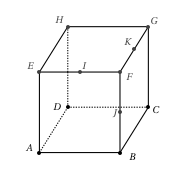
\includegraphics[scale=0.4]{images/exemple1.png}
\end{center}

\begin{itemize}
\pause \item {\color{blue} Question : Les droites $(IK)$ et $(AC)$ sont-elles parallèles ? sécantes ? }
\pause \item {\color{red} Réponse : $I$ milieu de $[EF]$ et $K$ milieu de $[FG]$ donc $(IK)//(EG)$ d'après la réciproque de Thalès. $\vect{EA}=\vect{FB}$ car $EFBA$ carré et  $\vect{FB}=\vect{GC}$ car $FBCG$ carré. Donc $\vect{EA}= \vect{GC}$ et donc $\vect{EG}=\vect{AC}$ et donc $(EG)//(AC)$. De $(EG)//(AC)$ et $(IK)//(EG)$, on déduit que $(IK)//(AC)$. $(IK)$ et $(AC)$ sont parallèles, donc elles ne sont pas sécantes.}
\end{itemize}


\end{frame}



\begin{frame}

\frametitle{Exemple 1 : Partie 3}

Figure dynamique sur \href{https://www.geogebra.org/m/ahkmk9br}{https://www.geogebra.org/m/ahkmk9br}.


\begin{center}
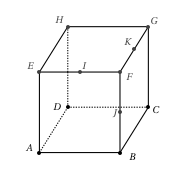
\includegraphics[scale=0.4]{images/exemple1.png}
\end{center}

\begin{itemize}
\pause \item {\color{blue} Question : La droite $(FG)$ coupe-t-elle le plan $(AEH)$ ? }
\pause \item {\color{red} Réponse : %On a $EFGH$ carré donc $(FG)//(EH)$. $(FG)$ est parallèle à une droite contenue dans le plan $(AEH)$ donc elle est parallèle au plan $(AEH)$. 
$(FG)$ contenue dans le plan $(BFG)$ qui est parallèle et non confondu avec le plan $(AEH)$ donc $(FG)$ ne coupe pas le plan $(AEH)$.
}
\end{itemize}


\end{frame}




\begin{frame}

\frametitle{Exemple 1 : Partie 4}

Figure dynamique sur \href{https://www.geogebra.org/m/ahkmk9br}{https://www.geogebra.org/m/ahkmk9br}.


\begin{center}
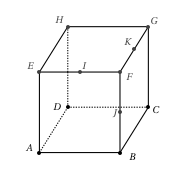
\includegraphics[scale=0.4]{images/exemple1.png}
\end{center}

\begin{itemize}
\pause \item {\color{blue} Question : Déterminer l'intersection du plan $(ABC)$ et du plan $(DHG)$.}
\pause \item {\color{red} Réponse :  Le plan $(DHG)$ est égal au plan $(DCG)$ et le plan $(ABC)$ est égal au plan $(ADC)$. La droite $(DC)$ appartient aux plans $(DCG)$ et $(ADC)$ qui ne sont pas confondus, la droite $(DC)$ est donc la droite d'intersection des plans  $(DCG)=(DHG)$ et $(ADC)=(ABC)$.
}
\end{itemize}


\end{frame}



\begin{frame}

\frametitle{Exemple 1 : Partie 5}

Figure dynamique sur \href{https://www.geogebra.org/m/ahkmk9br}{https://www.geogebra.org/m/ahkmk9br}.


\begin{center}
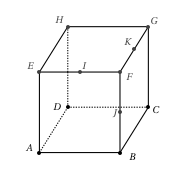
\includegraphics[scale=0.4]{images/exemple1.png}
\end{center}

\begin{itemize}
\pause \item {\color{blue} Question : Que pensez-vous de l'affirmation suivante  ?  $A_{0}$ : \og{} Si deux droites de l'espace  sont perpendiculaires à une même droite, alors elles sont parallèles. \og{}}
\pause \item {\color{red} Réponse :  Cette affirmation est fausse, comme le prouve le contre-exemple des droites $(EF)$ et $(FG)$ qui sont perpendiculaires à la droite $(BF)$ car $EFG$ et $BFGC$ sont des carrés, mais qui sont sécantes en $F$ et donc non parallèles.
}
\end{itemize}


\end{frame}




\begin{frame}

\frametitle{Exemple 1 : Partie 6}

Figure dynamique sur \href{https://www.geogebra.org/m/ahkmk9br}{https://www.geogebra.org/m/ahkmk9br}.


\begin{center}
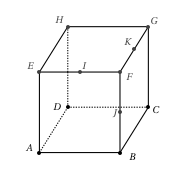
\includegraphics[scale=0.4]{images/exemple1.png}
\end{center}

\begin{itemize}
\pause \item {\color{blue} Question : Que pensez-vous de l'affirmation suivante ?  $A_{1}$ : \og{} Il existe un seul plan contenant les droites  $(CG)$ et $(BF)$. \og{} \og{}}
\pause \item {\color{red} Réponse :  Cette affirmation est vraie,  $BFGC$ est un carré donc $(GC)//(BF)$ et deux droites parallèles et non confondues définissent un plan. 
}
\end{itemize}


\end{frame}




\begin{frame}

\frametitle{Exemple 1 : Partie 7}

Figure dynamique sur \href{https://www.geogebra.org/m/ahkmk9br}{https://www.geogebra.org/m/ahkmk9br}.


\begin{center}
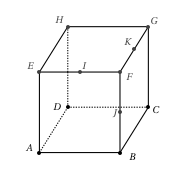
\includegraphics[scale=0.4]{images/exemple1.png}
\end{center}

\begin{itemize}
\pause \item {\color{blue}  Que pensez-vous de l'affirmation suivante ? $A_{2}$ :  \og{} Il existe un seul plan contenant les droites  $(FC)$ et $(BC)$. \fg{}}
\pause \item {\color{red} Réponse :  Cette affirmation est vraie, $(FC)$ et $(BC)$ sont deux droites sécantes, donc $B$, $F$ et $C$ sont trois points non alignés qui définissent un unique plan $(BFC)$ (on peut le nommer autrement). 
}
\end{itemize}


\end{frame}


\begin{frame}

\frametitle{Exemple 1 : Partie 8}

Figure dynamique sur \href{https://www.geogebra.org/m/ahkmk9br}{https://www.geogebra.org/m/ahkmk9br}.


\begin{center}
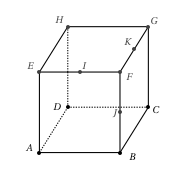
\includegraphics[scale=0.4]{images/exemple1.png}
\end{center}

\begin{itemize}
\pause \item {\color{blue}  Que pensez-vous de l'affirmation suivante ? $A_{3}$ : \og{} Il existe un seul plan contenant la droite $(CG)$. \fg{}}
\pause \item {\color{red} Réponse :  Cette affirmation est fausse, les plans $(DCG)$ et $(BCG)$ sont distincts et leur droite d'intersection est la droite $(CG)$. Il existe une infinité de plan contenant la droite $(CG)$.  
}
\end{itemize}


\end{frame}


\begin{frame}

\frametitle{Exemple 1 : Partie 9}

Figure dynamique sur \href{https://www.geogebra.org/m/ahkmk9br}{https://www.geogebra.org/m/ahkmk9br}.


\begin{center}
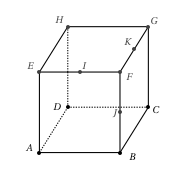
\includegraphics[scale=0.4]{images/exemple1.png}
\end{center}

\begin{itemize}
\pause \item {\color{blue}   Que pensez-vous de l'affirmation suivante ? $A_{4}$ : \og{} Il existe toujours un plan contenant quatre points de l'espace. \fg{}}
\pause \item {\color{red} Réponse :  Cette affirmation est fausse, comme le prouve le contre-exemple du tétraèdre $ABCF$ dont les quatre sommets ne peuvent être contenus dans un même plan.  
}
\end{itemize}


\end{frame}



\begin{frame}

\frametitle{Exemple 1 : Partie 10}

Figure dynamique sur \href{https://www.geogebra.org/m/ahkmk9br}{https://www.geogebra.org/m/ahkmk9br}.


\begin{center}
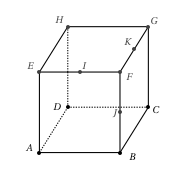
\includegraphics[scale=0.4]{images/exemple1.png}
\end{center}

\begin{itemize}
\pause \item {\color{blue}  Que pensez-vous de l'affirmation suivante ? $A_{5}$ : \og{} Il existe toujours un plan contenant trois points de l'espace. \fg{}}
\pause \item {\color{red} Réponse :  Cette affirmation est vraie,  soit trois points sont alignés ou confondus et il existe une droite (et une infinité de plans) ou une infinité de droites  (s'ils sont confondus) les contenant, soit ils ne sont pas alignés et il existe  un unique plan les contenant.
}
\end{itemize}


\end{frame}



\begin{frame}

\frametitle{Exemple 1 : Partie 11}

Figure dynamique sur \href{https://www.geogebra.org/m/ahkmk9br}{https://www.geogebra.org/m/ahkmk9br}.


\begin{center}
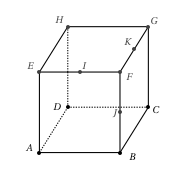
\includegraphics[scale=0.4]{images/exemple1.png}
\end{center}

\begin{itemize}
\pause \item {\color{blue}   Le point $B$ est-il l'intersection du plan $(EGB)$ et du plan $(ABC)$ ? }
\pause \item {\color{red} Réponse :  Cette affirmation est fausse,  si deux plans ont une intersection, ils sont soit confondus (ce qui n'est pas le cas de $(EGB)$ et  $(ABC)$), soit sécantes selon une droite. Dans les deux cas, si l'intersection de deux plans existent, elle comporte une infinité de points.
}
\end{itemize}


\end{frame}



\begin{frame}

\frametitle{Exemple 1 : Partie 12}

Figure dynamique sur \href{https://www.geogebra.org/m/ahkmk9br}{https://www.geogebra.org/m/ahkmk9br}.


\begin{center}
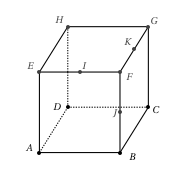
\includegraphics[scale=0.4]{images/exemple1.png}
\end{center}

\begin{itemize}
\pause \item {\color{blue}  Le point $B$ est-il l'intersection du plan $(EGB)$ et du plan $(ABC)$ ?}
\pause \item {\color{red} Réponse :  Cette affirmation est fausse,  si deux plans ont une intersection, ils sont soit confondus (ce qui n'est pas le cas de $(EGB)$ et  $(ABC)$), soit sécantes selon une droite. Dans les deux cas, si l'intersection de deux plans existent, elle comporte une infinité de points.
}
\end{itemize}


\end{frame}




\begin{frame}

\frametitle{Exemple 1 : Partie 13}

Figure dynamique sur \href{https://www.geogebra.org/m/ahkmk9br}{https://www.geogebra.org/m/ahkmk9br}.


\begin{center}
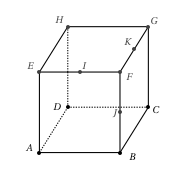
\includegraphics[scale=0.4]{images/exemple1.png}
\end{center}

\begin{itemize}
\pause \item {\color{blue}   Citer un plan contenant la droite $(BG)$, un plan parallèle à la droite $(BG)$ mais ne la contenant pas et un plan sécant à la droite $(BG)$.}
\pause \item {\color{red} Réponse :  Le plan $(BCG)$ contient la droite $(BG)$, le plan $(ADH)$ est parallèle à la droite $(BG)$ et le plan $(CDG)$ est sécante à la droite $(BG)$ en $G$. 
}
\end{itemize}


\end{frame}




\begin{frame}

\frametitle{Exemple 1 : Partie 14}


\begin{center}
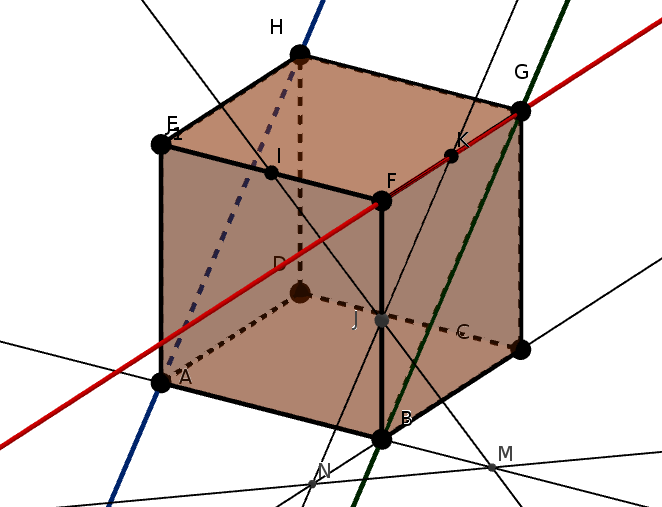
\includegraphics[scale=0.1]{images/exemple1-intersection.png}
\end{center}

\begin{itemize}
\pause \item {\color{blue}   Les plans $(IJK)$ et $(ABC)$ sont-ils sécants ? Si oui, déterminer leur intersection.}
\pause \item {\color{red} Réponse : Dans le plan $(ABF)$, les droites $(IJ)$ et $(AB)$ sont sécantes en un point $M$, qui appartient à l'intersection des plans $(IJK)$ et du plan $(ABC)$ car $(IJ) \subset (IJK)$ et $(AB) \subset (ABC)$. Dans le plan $(BFC)$, les droites $(KJ)$ et $(BC)$ sont sécantes en un point $N$, qui appartient à l'intersection à l'intersection des plans $(IJK)$ et du plan $(ABC)$ car $(JK) \subset (IJK)$ et $(BC) \subset (ABC)$. On en déduit que la droite $(MN)$ appartient à l'intersection des plans $(IJK)$ et $(ABC)$, de plus ces deux plans ne sont pas confondus donc ils sont sécants selon la droite $(MN)$.
}
\end{itemize}


\end{frame}


\begin{frame}

\frametitle{Exemple 2 : Partie 1}


\begin{center}
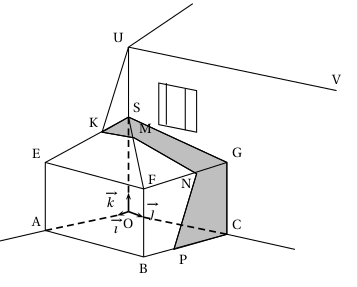
\includegraphics[scale=0.25]{images/exemple2.png}
\end{center}

\begin{itemize}
\pause \item {\color{blue}   Les plans $(SEF)$ et $(UKV)$ sont sécants selon la droite $(KM)$. De plus la droite $(RF)$ incluse dans le plan $(SEF)$ est parallèle à la droite $(UV)$ incluse dans le plan $(UKV)$. D'après le théorème du toit, les droites $(UV)$,  $(EF)$ et $(KM)$ sont parallèles.}

\end{itemize}
\end{frame}



\begin{frame}

\frametitle{Exemple 2 : Partie 2}


\begin{center}
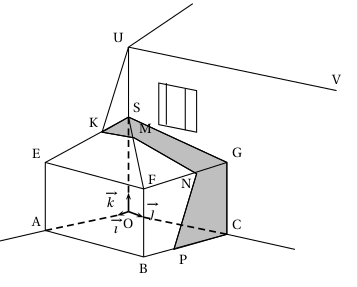
\includegraphics[scale=0.25]{images/exemple2.png}
\end{center}

\begin{itemize}
\pause \item {\color{blue}   Les plans $(SOA)$ et $(GCB)$ sont parallèles. Le plan $(UVK)$ coupe $(SOA)$ selon la droite  $(UK)$ et $(GCB)$ selon la droite $(NP)$. D'après une propriété du cours, un plan coupe deux plans parallèles selon des droites parallèles donc $(UK)//(NP)$.}
\end{itemize}
\end{frame}






\begin{frame}

\label{exemple3}

\frametitle{Construction d'une section plane de cube Partie 1 }

\begin{block}



Soit $ABCDEFGH$ un cube dont on veut construire la section par un plan $\mathcal{P}$.

\begin{itemize}
	\item \textbf{Étape 1 :} On a deux alternatives :
	
	\begin{itemize}
\pause	\item On choisit deux points de $\mathcal{P}$ situés également   dans le plan d'une face   $\mathcal{F}$ du cube et on trace la droite $\mathcal{D}$ qui les relie.
	
	On construit alors les points intersections de cette droite $\mathcal{D}$ avec les droites portant les  arêtes de cette face  $\mathcal{F}$   du cube.
 
	\pause \item Si on connaît déjà la droite $\mathcal{D}$  d'intersection de $\mathcal{P}$ avec le plan d'une face $ \mathcal{F}_{1}$  du cube, la droite d'intersection de $\mathcal{P}$  avec la face parallèle $\mathcal{F}_{2}$  est nécessairement parallèle à $\mathcal{D}$. Pour la tracer il suffit de connaître un point de $\mathcal{P}$  appartenant aussi au plan de la face $\mathcal{F}_{2}$. 
	
	\end{itemize}
	
\end{itemize}
\end{block}


\end{frame}



\begin{frame}



\frametitle{Construction d'une section plane de cube Partie 2 }

\begin{block}



Soit $ABCDEFGH$ un cube dont on veut construire la section par un plan $\mathcal{P}$.

\begin{itemize}

		\item \textbf{Étape 2 :} On vérifie si on peut refermer un polygone dont les côtés relient des points intersections du plan $\mathcal{P}$  avec les différentes arêtes du cube donnés initialement ou obtenus lors des étapes précédentes. 
		
		Si c'est le cas, ce polygone fermé (avec au plus $6$ côtés) est la section du cube par le plan $\mathcal{P}$, sinon on recommence à l'\textbf{Étape 1} .	
\end{itemize}
\end{block}


\end{frame}



\begin{frame}



\frametitle{Construction d'une section plane, exemple 3}


Dérouler le protocole de construction de la figure dynamique \href{https://www.geogebra.org/m/vhnydz7z}{https://www.geogebra.org/m/vhnydz7z} à partir de l'étape 9.

\end{frame}



\begin{frame}
\label{exemple4}


\frametitle{Construction d'une section plane, exemple 4, Question 1}


Dérouler le protocole de construction de la figure dynamique \href{https://www.geogebra.org/m/pgehdq4f}{https://www.geogebra.org/m/pgehdq4f} à partir de l'étape 11.

\end{frame}




\begin{frame}



\frametitle{Construction d'une section plane, exemple 4, Question 2}


Dérouler le protocole de construction de la figure dynamique \href{https://www.geogebra.org/m/cmwhrsty}{https://www.geogebra.org/m/cmwhrsty} à partir de l'étape 12.

\end{frame}



\begin{frame}

\label{exemple5}

\frametitle{Exemple 5, Partie 1}


\begin{center}
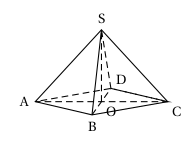
\includegraphics[scale=0.5]{images/exemple5.png}
\end{center}

\begin{itemize}
\pause \item {\color{blue} Question : Démontrer
que  (SO) est orthogonale à (ABC).}
\pause \item {\color{red} Réponse :  Dans le plan $(SAC)$, $SA=SC$  car $SA=SB=SC$ et $O$ milieu de $[AC]$ donc $(SO)$ médiatrice de $[AC]$ donc $(SO) \perp (AC)$. Dans le plan $(SBD)$, $SB=SD$  car $SB=SC=SD$ et $O$ milieu de $[BD]$ donc $(SO)$ médiatrice de $[BD]$ donc $(SO) \perp (BD)$. $(SO)$ est orthogonale à deux droites sécantes du plan  $(ABC)$,  $(AC)$ et $(BD)$, donc $(SO)$ orthogonale au plan $(ABC)$.
}
\end{itemize}



\end{frame}


\begin{frame}



\frametitle{Exemple 5, Partie 2}


\begin{center}
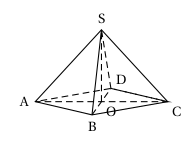
\includegraphics[scale=0.5]{images/exemple5.png}
\end{center}

\begin{itemize}
\pause \item {\color{blue} Question : En déduire le volume, en cm$^3$, de la pyramide SABCD.}
\pause \item {\color{red} Réponse : Le volume de la pyramide SABCD s'obtient en prenant le tiers du produit de l'aire de la base ABCD par la hauteur SO.  AC = 24 donc le côté AB du carré mesure $24/\sqrt{2}$ et son aire est égale à $24^{2}/2= 288$. De plus SOA rectangle en O donc d'après le théorème de  Pythagore, $SO^{2}=SA^{2}-OA^{2}=24^{2}/2 - (24/2)^{2}=12^{2}$ donc $SO=12$. Le volume de la pyramide est donc  de $\frac{1}{3} \times 12 \times 288=1152$.
}
\end{itemize}



\end{frame}


\begin{frame}



\label{exemple6}

\frametitle{Exemple 6, Partie 2}


\begin{center}
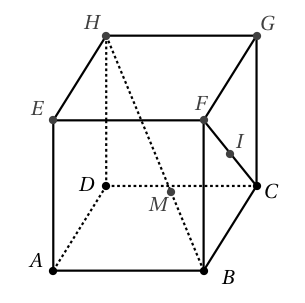
\includegraphics[scale=0.1]{images/exemple6.png}
\end{center}

\begin{itemize}
 \item D'après la relation de Chasles, $\vect{FM}=\vect{FH}+\vect{HM}=\vect{FH}+\frac{2}{3}\vect{HB}$.
On a donc : $\vect{FM}= \vect{FH}+\frac{2}{3}(\vect{HD}+\vect{DB})= \vect{BD}+\frac{2}{3}(\vect{HD}+\vect{DB})=\frac{1}{3}\vect{BD}-\frac{2}{3}\vect{AE}=\frac{1}{3}(\vect{BA}+\vect{AD})-\frac{2}{3}\vect{AE}=\frac{1}{3}(-\vect{AB}+\vect{AD}-2\vect{AE})$.
\end{itemize}



\end{frame}




\begin{frame}



\frametitle{Exemple 6, Partie 3}


\begin{center}
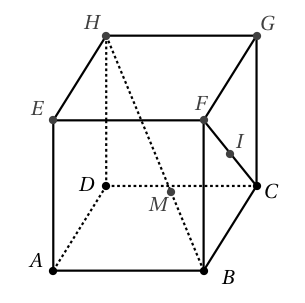
\includegraphics[scale=0.1]{images/exemple6.png}
\end{center}

\begin{itemize}
\item On a $\vect{AM}=\vect{AB}+\vect{BM}=\vect{AB}+\frac{1}{3}\vect{BH}=\vect{AB}+\frac{1}{3}(\vect{BA} + \vect{AD} + \vect{AE})=\frac{1}{3}(2\vect{AB}+\vect{AD} + \vect{AE}  )$.

Par ailleurs, $\vect{AI}=\vect{AB}+\frac{1}{2}\vect{BG}=\vect{AB}+\frac{1}{2}(\vect{AD}+\vect{AE})=\frac{1}{2}(2\vect{AB}+\vect{AD}+\vect{AE})$.

On en déduit que $\vect{AM}=\frac{2}{3}\vect{AI}$, les vecteurs $\vect{AM}$ et $\vect{AI}$ sont donc colinéaires et les points $A$, $M$ et$I$ sont alignés.
\end{itemize}



\end{frame}


\begin{frame}



\frametitle{Exemple 6, Partie 4}


\begin{center}
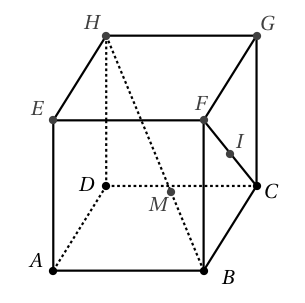
\includegraphics[scale=0.1]{images/exemple6.png}
\end{center}

\begin{itemize}

\item On a $\vect{AM}=\vect{AB}+\vect{BM}=\vect{AB}+\frac{1}{3}\vect{BH}=\vect{AB}+\frac{1}{3}(\vect{BA} + \vect{AD} + \vect{AE})=\frac{1}{3}(2\vect{AB}+\vect{AD} + \vect{AE}  )$.

Par ailleurs, $\vect{AI}=\vect{AB}+\frac{1}{2}\vect{BG}=\vect{AB}+\frac{1}{2}(\vect{AD}+\vect{AE})=\frac{1}{2}(2\vect{AB}+\vect{AD}+\vect{AE})$.

On en déduit que $\vect{AM}=\frac{2}{3}\vect{AI}$, les vecteurs $\vect{AM}$ et $\vect{AI}$ sont donc colinéaires et les points $A$, $M$ et$I$ sont alignés.
\end{itemize}



\end{frame}




\begin{frame}



\label{exemple7}

\frametitle{Exemple 7, Partie 1}

L'espace est muni d'un repère \Oijk.  Soient les points $A\Coordesp{-1}{3}{4}$, $B\Coordesp{7}{6}{1}$ et $C\Coordesp{0}{2}{-5}$.


\begin{itemize}
\pause \item {\color{blue} Question :  Calculer les coordonnées du point $D$ tel que $ABCD$ est un parallélogramme.  }
\pause \item {\color{red} Réponse : $ABCD$ est un parallélogramme donc $\vect{BC}=\vect{AD}$. Or $\vect{BC}\coordesp{-7}{-4}{-6}$ et si on note $D\coordesp{x}{y}{z}$ on a  $\vect{AD}\coordesp{x+1}{y-3}{z-4}$.  $\vect{BC}=\vect{AD} \Leftrightarrow \Sys{x+1=-7}{y-3=-4}{z-4=-6} \Leftrightarrow \Sys{x=-8}{y=-1}{z=-2}$.
}
\end{itemize}



\end{frame}




\begin{frame}


\frametitle{Exemple 7, Partie 2}

L'espace est muni d'un repère \Oijk.  Soient les points $A\Coordesp{-1}{3}{4}$, $B\Coordesp{7}{6}{1}$ et $C\Coordesp{0}{2}{-5}$.


\begin{itemize}
 \item {\color{blue} Question :  Calculer les coordonnées du point $F$ symétrique de $D$ par rapport à $A$. }
\pause \item {\color{red} Réponse : $A$ milieu de $[FD]$ donc  les coordonnées de $F\coordesp{x}{y}{z}$ vérifient :  
 $\Sys{(x+x_{D})/2=x_{A}}{(y+y_{D})/2=y_{A}}{(z+z_{D})/2=z_{A}} \Leftrightarrow \Sys{x=6}{y=7}{z=10}$.  On a donc $F\coordesp{x=6}{y=7}{z=10}$.
}
\end{itemize}



\end{frame}


\begin{frame}


\frametitle{Exemple 7, Partie 3}

L'espace est muni d'un repère \Oijk.  Soient les points $A\Coordesp{-1}{3}{4}$, $B\Coordesp{7}{6}{1}$ et $C\Coordesp{0}{2}{-5}$.


\begin{itemize}
 \item {\color{blue} Question :  Les points $G\Coordesp{5}{2}{3}$, $H\Coordesp{-1}{3}{2}$ et $I\Coordesp{-7}{4}{1}$ sont-ils alignés ?
}
\pause \item {\color{red} Réponse :  $\vect{GH}\coordesp{-6}{1}{-1}$  et  $\vect{HI}\coordesp{-6}{1}{-1}$ . On remarque que  $\vect{GH}= \vect{HI}$ donc $H$ est le milieu de $[GI]$ et $G$, $H$ et $I$ sont alignés.
}
\end{itemize}



\end{frame}


\begin{frame}


\frametitle{Exemple 7, Partie 4}

L'espace est muni d'un repère \Oijk.  Soient les points $A\Coordesp{-1}{3}{4}$, $B\Coordesp{7}{6}{1}$ et $C\Coordesp{0}{2}{-5}$.


\begin{itemize}
 \item {\color{blue} Question :  Montrer que les points $J\Coordesp{-4}{5}{-1}$, $K\Coordesp{-1}{5}{-4}$, $L\Coordesp{-2}{12}{4}$ et $M\Coordesp{4}{12}{-2}$ sont coplanaires.
}
\pause \item {\color{red} Réponse :  On calcule les coordonnées de trois vecteurs de même origine $J$ :  $\vect{JK}\coordesp{3}{0}{-3}$, $\vect{JL}\coordesp{2}{7}{5}$  et $\vect{JM}\coordesp{8}{7}{-1}$. On remarque que $\vect{JM}=\vect{JL}+2\vect{JK}$, on peut en déduire que $\vect{JM}$, $\vect{JL}$ et $\vect{JLK}$ sont coplanaires et que les points $J$, $L$, $L$ et $M$ appartiennent au même plan. 
}
\end{itemize}



\end{frame}



\begin{frame}

\label{exemple8}

\frametitle{Exemple 8, Partie 1}

Soit $\mathcal{D}$ la droite de représentation paramétrique : $\left\{\begin{array}{l} x=4-3t \\ y=2t-1 \\ 4z=8+t \end{array} \right.\ , \ t\in\R$


\begin{itemize}
 \item {\color{blue} Question :  Déterminer les coordonnées d'un point de $\mathcal{D}$ et un vecteur directeur de $\mathcal{D}$.
}
\pause \item {\color{red} Réponse :  

$$\left\{\begin{array}{l} x=4-3t \\ y=2t-1 \\ 4z=8+t \end{array} \right. \Leftrightarrow  \left\{\begin{array}{l} x=4-3t \\ y=-1+2t \\ z=2+0,25t \end{array} \right. \ t\in\R $$
Un point de $\mathcal{D}$ est $E\coordesp{4}{-1}{2}$ et un vecteur directeur est $\vect{u}\coordesp{-3}{2}{0,25}$.
}

\end{itemize}



\end{frame}



\begin{frame}


\frametitle{Exemple 8, Partie 2}

Soit $\mathcal{D}$ la droite de représentation paramétrique : $\left\{\begin{array}{l} x=4-3t \\ y=2t-1 \\ 4z=8+t \end{array} \right.\ , \ t\in\R$


\begin{itemize}
 \item {\color{blue}  Le point $A\Coordesp{19}{-11}{7}$ appartient-il à $\mathcal{D}$ ?
}
\pause \item {\color{red} Réponse : on résout un système d'équations :  

$$\left\{\begin{array}{l} 19=4-3t \\ -11=2t-1 \\ 7=2+0,5t\end{array} \right. \Leftrightarrow  \left\{\begin{array}{l} t=-5 \\ t=-5 \\ t=20 \end{array} \right. \ t\in\R $$
Ce système n'a pas de solution, donc le point $A\Coordesp{19}{-11}{7}$  n'appartient à la droite $\mathcal{D}$.
}

\end{itemize}



\end{frame}



\begin{frame}


\frametitle{Exemple 8, Partie 3}

 $\mathcal{D}$ droite de représentation paramétrique : $\left\{\begin{array}{l} x=4-3t \\ y=2t-1 \\ 4z=8+t \end{array} \right.\ , \ t\in\R$


\begin{itemize}
 \item {\color{blue} Soient $B\Coordesp{3}{2}{-1}$ et $C\Coordesp{-9}{7}{0}$.

La droite $(BC)$ est-elle parallèle à  $\mathcal{D}$ ?  
}
\pause \item {\color{red} Réponse : Un vecteur directeur de la droite $(BC)$ est $\vect{BC}\coordesp{-12}{5}{1}$. Un vecteur directeur de la droite $\mathcal{D}$ est $\vect{u}\coordesp{-3}{2}{0,25}$. }

\pause \item {\color{red} $(BC)$ et $\mathcal{D}$ sont parallèles si et seulement si $\vect{u}$ et $\vect{BC}$ sont colinéaires.
$\vect{u}$ et $\vect{BC}$ sont colinéaires si et seulement s'il existe un réel $\lambda $ tel que $\vect{u}= \lambda \vect{BC}$.

$\vect{u}= \lambda \vect{BC} \Leftrightarrow \Sys{-3=-12\lambda}{2=5\lambda }{0,25=\lambda} \Leftrightarrow  \Sys{0,25=\lambda}{0,4=\lambda }{0,25=\lambda}$.

Système sans solution donc  $\vect{u}$ et $\vect{BC}$ ne sont pas colinéaires.
}

\end{itemize}



\end{frame}




\begin{frame}


\frametitle{Exemple 8, Partie 4}

 Soient $B\Coordesp{3}{2}{-1}$ et $C\Coordesp{-9}{7}{0}$.


\begin{itemize}
 \item {\color{blue} Représentation paramétrique de la droite $(BC)$ ? 
}
\pause \item {\color{red} Réponse :  $\vect{BC}\coordesp{-12}{5}{1}$ donc une représentation paramétrique de la droite $(BC)$ est : 

$\left\{\begin{array}{l} x=3-12u \\ y=2 + 5u\\ z=-1+u \end{array} \right.\ , \ u\in\R$
}

\end{itemize}



\end{frame}



\begin{frame}


\frametitle{Exemple 8, Partie 5}

\begin{itemize}
 \item {\color{blue} Question : $(BC)$  et $\mathcal{D}$ sont-elles sécantes ? 
}
\pause \item {\color{red} Réponse :  On a déjà démontré que  $(BC)$  et $\mathcal{D}$ ne sont pas parallèles, donc  $(BC)$  et $\mathcal{D}$ sont soit sécantes soit non coplanaires. Il suffit de déterminer si elles ont un point d'intersection en résolvant le système d'inconnues $x$, $y$, $z$, $t$, $u$ :

$\Sys{x=3-12u=4-3t}{y=2 + 5u=2t-1}{z=-1+u=2+0,25t}$.
 
On élimine d'abord $x$, $y$ et $z$ pour résoudre en $u$ et $t$ par substitution :

$\Sys{3-12u=4-3t}{2 + 5u=2t-1}{-1+u=2+0,25t}\Leftrightarrow \Sys{3-36-3t=4-3t}{2+15+1,25t=2t-1}{u=3+0,25t}$ 

}

\end{itemize}



\end{frame}



\begin{frame}


\frametitle{Exemple 8, Partie 6}

\begin{itemize}
 \item {\color{blue} Question : $(BC)$  et $\mathcal{D}$ sont-elles sécantes ? 
}
\pause \item {\color{red} $\Sys{3-12u=4-3t}{2 + 5u=2t-1}{-1+u=2+0,25t}\Leftrightarrow \Sys{3-36-3t=4-3t}{2+15+1,25t=2t-1}{u=3+0,25t}$ 
$\Leftrightarrow \Sys{-33=4}{2+15+1,25t=2t-1}{u=3+0,25t}$


La première équation n'a pas de solution, donc le système n'a pas de solution, donc $(BC)$  et $\mathcal{D}$ ne sont pas sécantes. Comme elles ne sont pas parallèles, elles sont donc non coplanaires.

}

\end{itemize}



\end{frame}




\end{document}